\documentclass{lab_sheet}
\usepackage{longtable}
\def\ddfrac#1#2{\displaystyle\frac{\displaystyle #1}{\displaystyle #2}}

\begin{document}
    \titlePage{Familiarization with Basic CT/DT Functions}{December 5, 2021}
\section{Objectives}
\begin{itemize}
    \item Familiarization and review of basic continuous time and discrete time functions.
\end{itemize}
\section{Background Theory}
\subsection{Some MATLAB commands}
\begin{longtable}[H]
    {|m{0.2\linewidth}|m{0.7\linewidth}|}
        \hline
        \textbf{Command}&\textbf{Use Case}\\
        \hline\hline
        \texttt{who}&Lists current variables\\
        \hline
        \texttt{whos}&Lists current variables (long display)\\
        \hline
        \texttt{input}&Requests user input\\
        \hline
        \texttt{disp}&Displays contents of an array or string\\
        \hline
        \texttt{clear all}&Remove variables from the current workspace\\
        \hline
        \texttt{close all}&Close all plots\\
        \hline
        \texttt{pause}&Pause execution\\
        \hline
        \texttt{home}&Send cursor home\\
        \hline
        \texttt{length}&Computes number of elements\\
        \hline
        \texttt{plot}&Generates xy plot\\
        \hline
        \texttt{tiledlayout}&Creates a tiled chart layout for displaying multiple plots\\
        \hline
        \texttt{nexttile}&Creates an axes object and places it into the next empty tile\\
        \hline
        \texttt{hold}&Freezes current plot\\
        \hline
        \texttt{grid}&Displays grid lines\\
        \hline
        \texttt{stem}&Creates stem plot\\
        \hline
        \texttt{legend}&Places legend on figure\\
        \hline
        \texttt{xlabel}&Adds text label to x-axis\\
        \hline
        \texttt{ylabel}&Adds text label to y-axis\\
        \hline
        \texttt{real}&Real part of complex number\\
        \hline
        \texttt{imag}&Imaginary part of complex number\\
        \hline
        \texttt{abs}&Absolute value and
        complex magnitude\\
        \hline
        \texttt{angle}&Phase angle in interval $[-\pi,\pi]$\\
        \hline
        \texttt{zeros}&Creates an array of zeros\\
        \hline
        \texttt{ones}&Creates an array of ones\\
        \hline
        \texttt{exp}&Returns the exponential of arguments\\
        \hline
        \texttt{sin}&Returns the sine of argument in
        radians\\
        \hline
        \texttt{cos}&Returns the cosine of argument in
        radians\\
       \hline
       \caption{Some MATLAB commands with their use cases}
\end{longtable}
\section{Lab Exercises}
\problem{Plot the baic signal using MATLAB}
\subproblem{Impulse Response}
\matlabcode{impulse_response}{Matlab function to return impulse response}
\subproblem{Unit-step}
\matlabcode{unit_response}{Matlab function to return unit-step response}
\subproblem{Ramp}
\matlabcode{ramp_response}{Matlab function to return ramp response}
\subproblem{Rectangular}
\matlabcode{rectangular_response}{Matlab function to return rectangular response}
\matlabcode{basic_plot_selector}{Matlab function to return desired response based on user input}
\matlabcode{lab_2_1}{Matlab script to plot desired response based on user input}

\begin{verbatim}
    >> lab_2_1
    Enter function you want to plot: impulse
\end{verbatim}
\begin{figure}[H]
    \centering
    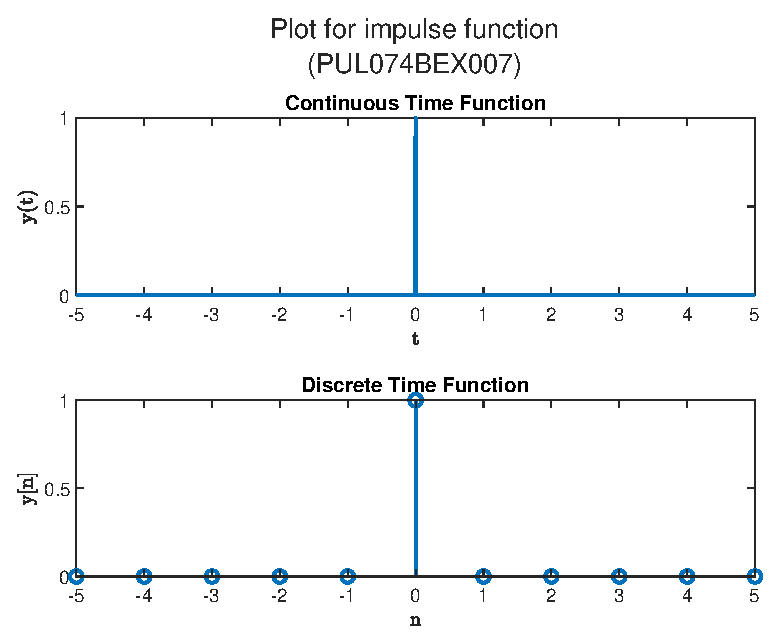
\includegraphics[width=0.85\linewidth]{../Figures/impulse.eps}
    \caption{Plot for impulse function}
    \label{fig:2_1_a}
\end{figure}
\pagebreak
\begin{verbatim}
    >> lab_2_1
    Enter function you want to plot: unit-step
\end{verbatim}
\begin{figure}[H]
    \centering
    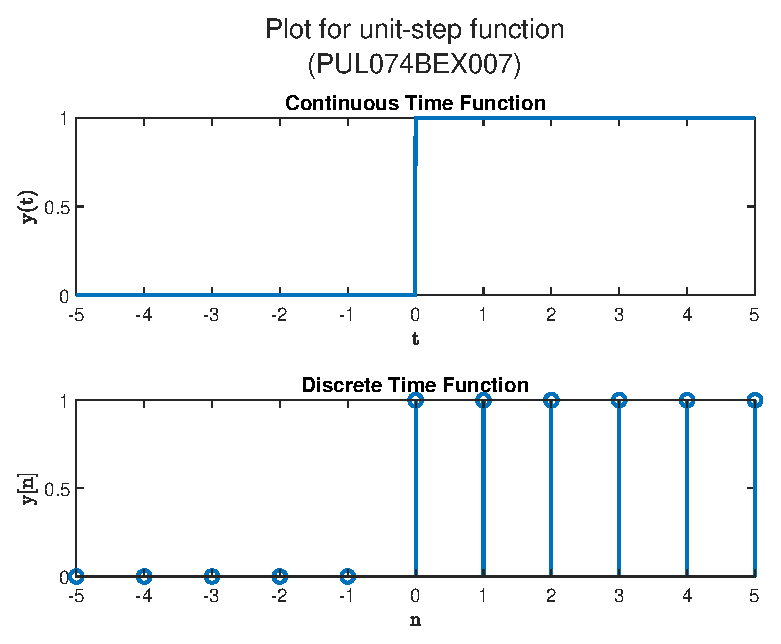
\includegraphics[width=0.85\linewidth]{../Figures/unit-step.eps}
    \caption{Plot for unit-step function}
    \label{fig:2_1_b}
\end{figure}

\pagebreak
\begin{verbatim}
    >> lab_2_1
    Enter function you want to plot: ramp
\end{verbatim}
\begin{figure}[H]
    \centering
    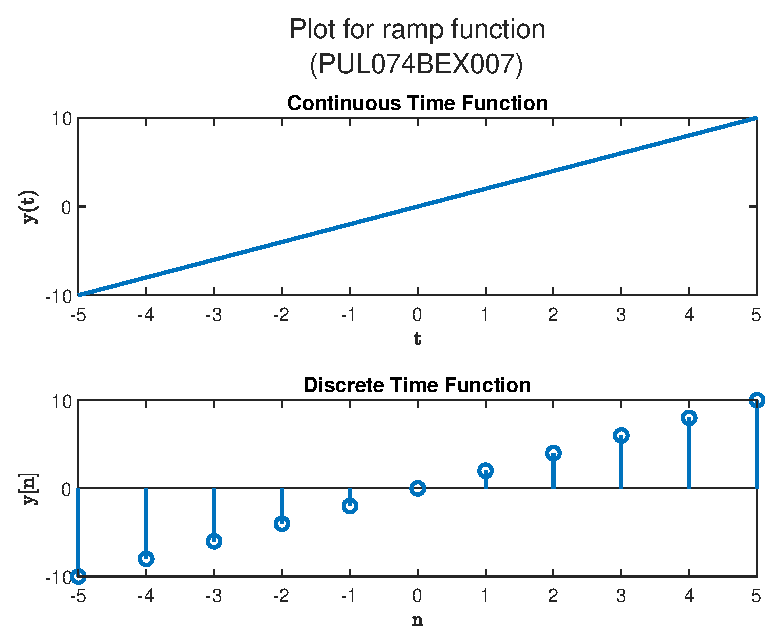
\includegraphics[width=0.85\linewidth]{../Figures/ramp.eps}
    \caption{Plot for ramp function}
    \label{fig:2_1_c}
\end{figure}
\pagebreak
\begin{verbatim}
    >> lab_2_1
    Enter function you want to plot: rectangular
\end{verbatim}

\begin{figure}[H]
    \centering
    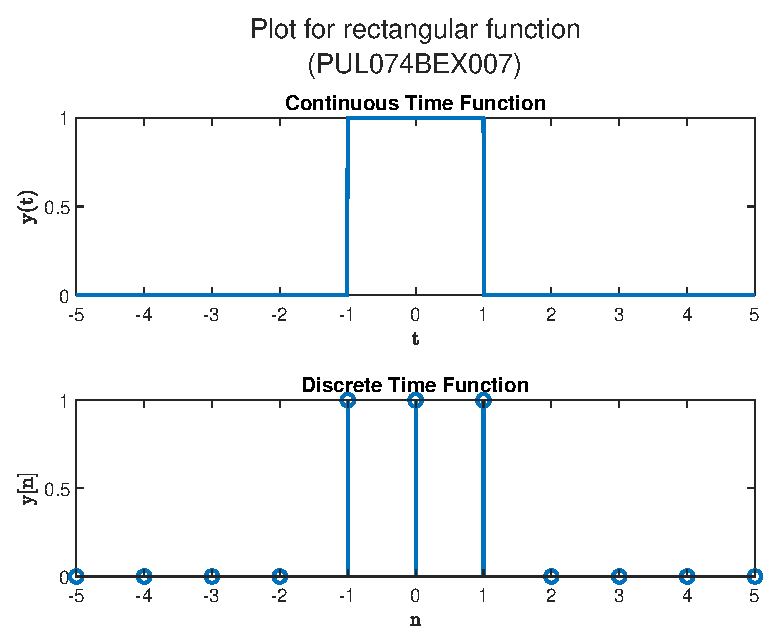
\includegraphics[width=0.85\linewidth]{../Figures/rectangular.eps}
    \caption{Plot for rectangular function}
    \label{fig:2_1_d}
\end{figure}

\problem{Plot the following continuous-time signals.}
\subproblem{$x(t)=Ce^{at}$ where $C$ and $a$ are real numbers and choose $C$ and $a$ both positive and negative.} 
\matlabcode{exponential_response_ct}{Matlab function to return CT exponential response}
\matlabcode{lab_2_2_a}{Matlab script to plot CT exponential function with $C$ and $a$ both real}
\begin{figure}[H]
    \centering
    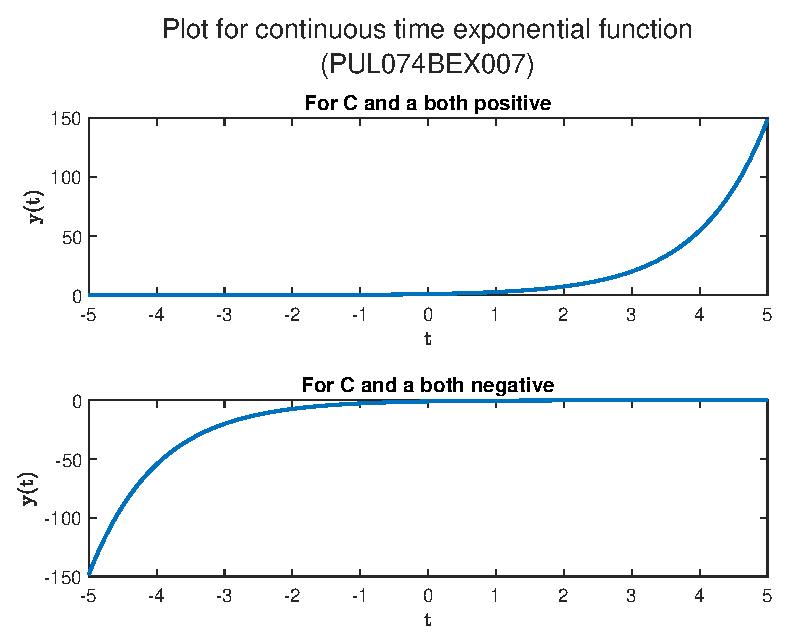
\includegraphics[width=0.835\linewidth]{../Figures/lab_2_2_a.eps}
    \caption{Plot for CT exponential function with $C$ and $a$ both real}
    \label{fig:2_2_a}
\end{figure}
\subproblem{Plot the same signal taking $a$ as pure imaginary number.}
\matlabcode{lab_2_2_b}{Matlab script to plot CT exponential function with $a$ purely imaginary}
\begin{figure}[H]
    \centering
    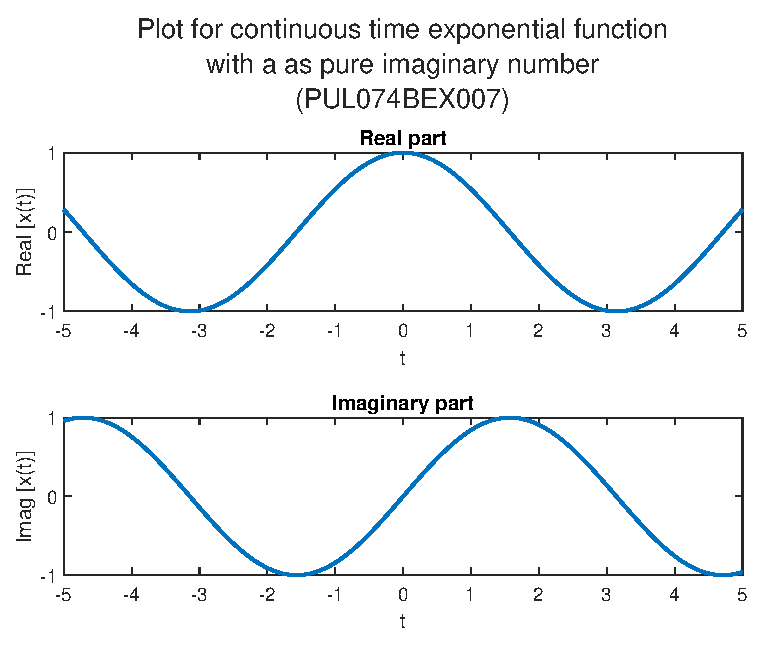
\includegraphics[width=0.835\linewidth]{../Figures/lab_2_2_b.eps}
    \caption{Plot for CT exponential function with $C$, $a$ both positive and negative}
    \label{fig:2_2_b}
\end{figure}
\subproblem{Consider complex exponential signal as specified in b) where $C$ is expressed in polar form i.e., $C=|C|e^{j\theta}$ and $a$ in rectangular form i.e., $a=r+j\omega_o$. Then function $x(t)$, on simplification, becomes $$ x(t)= |C|e^{rt}[\cos(\omega_o t+\theta)+j\sin(\omega_o t+\theta)]$$
Now, plot the signal for different values of r and comment on the results.\\
i. r=0 \quad \quad ii. r<0 \quad \quad iii. r>0
}
\matlabcode{exponential_response_polar}{Matlab function to return CT exponential (polar form) response}
\matlabcode{lab_2_2_c}{Matlab script to plot the function for values of $r$ based on user input}
\pagebreak
\begin{verbatim}
    >> lab_2_2_c
    Enter the value for r: 0
\end{verbatim}

\begin{figure}[H]
    \centering
    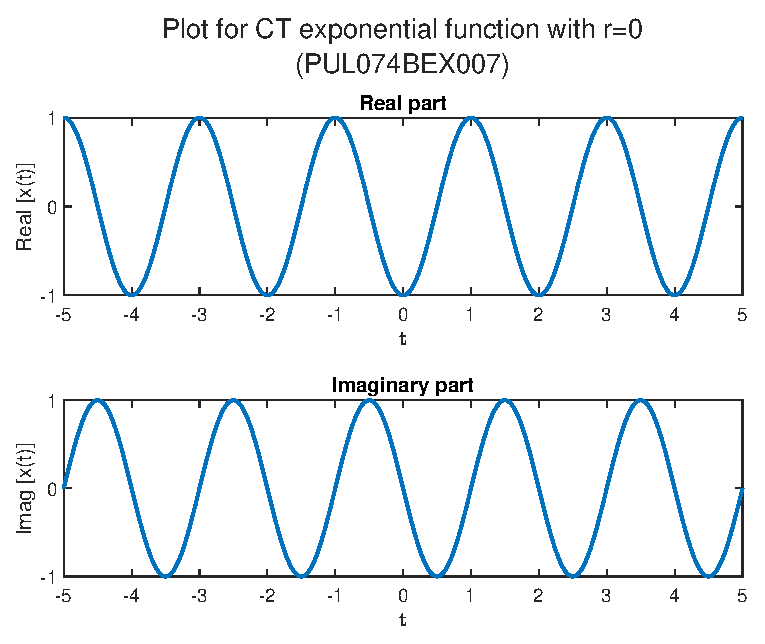
\includegraphics[width=0.85\linewidth]{../Figures/lab_2_2_c_0.eps}
    \caption{Plot for CT exponential function with $r=0$}
    \label{fig:2_2_c_0}
\end{figure}
\pagebreak
\begin{verbatim}
    >> lab_2_2_c
    Enter the value for r: -1
\end{verbatim}

\begin{figure}[H]
    \centering
    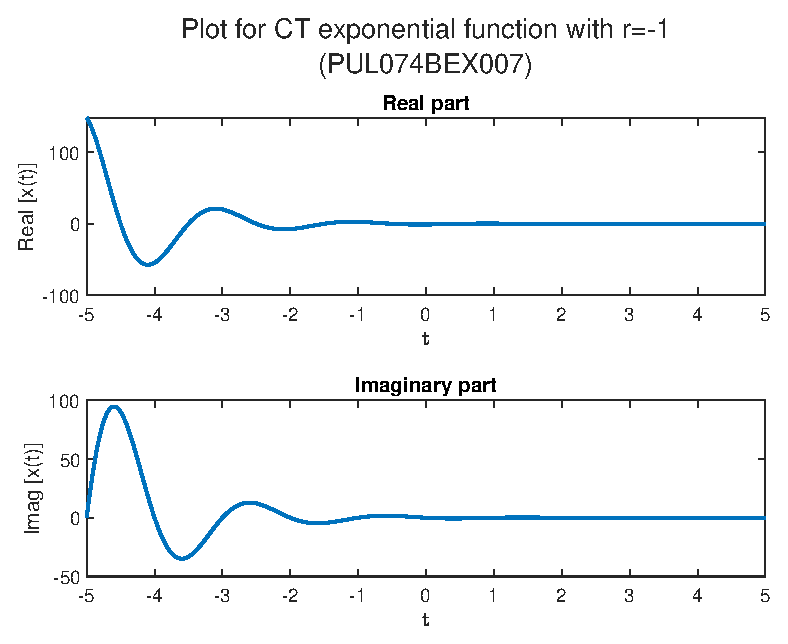
\includegraphics[width=0.85\linewidth]{../Figures/lab_2_2_c_-1.eps}
    \caption{Plot for CT exponential function with $r=-1$}
    \label{fig:2_2_c_-1}
\end{figure}
\pagebreak
\begin{verbatim}
    >> lab_2_2_c
    Enter the value for r: 1
\end{verbatim}

\begin{figure}[H]
    \centering
    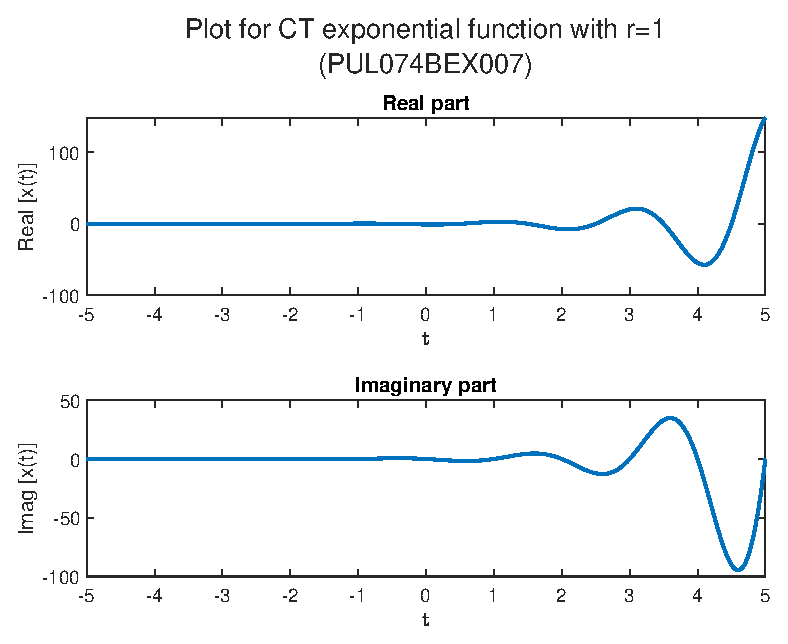
\includegraphics[width=0.85\linewidth]{../Figures/lab_2_2_c_1.eps}
    \caption{Plot for CT exponential function with $r=-1$}
    \label{fig:2_2_c_1}
\end{figure}

\problem{Plot the DT exponential function $x[n]=a^n$, $a=|a|e^{j\theta}$. Choose the suitable value of $a$ and $\theta$.}
\matlabcode{exponential_response_dt}{Matlab function to return DT exponential response}
\matlabcode{lab_2_3}{Matlab script to plot DT exponential function}
\begin{figure}[H]
    \centering
    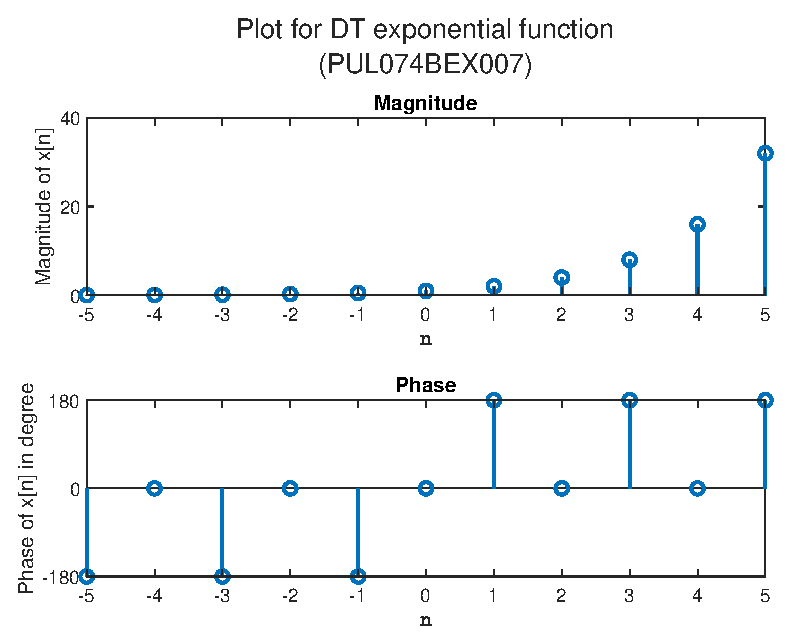
\includegraphics[width=0.85\linewidth]{../Figures/lab_2_3.eps}
    \caption{Plot for DT exponential function}
    \label{fig:2_3}
\end{figure}
\problem{Synthesize the signal from the FS coefficients as $C_0=1$, $C_1=C_{-1}=\ddfrac{1}{4}$, $C_2=C_{-2}=\ddfrac{1}{2}$, $C_3=C_{-3}=\ddfrac{1}{3}$.}
\matlabcode{synthesize_signal}{Matlab function to return synthesized signal from the FS coefficients}
\matlabcode{lab_2_4}{Matlab script to plot the synthesized signal}
\begin{figure}[H]
    \centering
    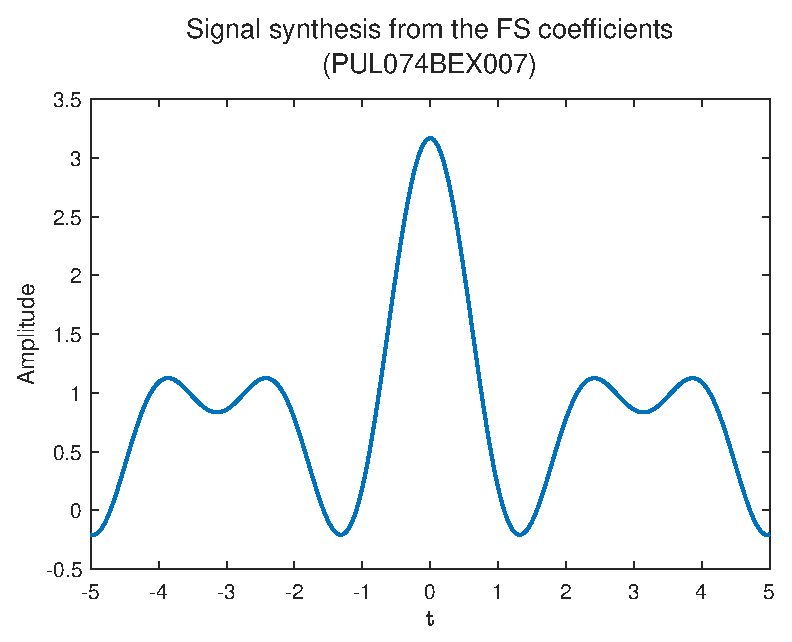
\includegraphics[width=0.85\linewidth]{../Figures/lab_2_4.eps}
    \caption{Plot for synthesized signal from the FS coefficients}
    \label{fig:2_4}
\end{figure}
\problem{Plot fundamental sinusoidal signal, its higher harmonics up to 5\textsuperscript{th} harmonics and add all of them
to see the result. Comment on the result.}
\matlabcode{harmonic_sum}{Matlab function to return sinusoidal harmonics and their sum}
\matlabcode{lab_2_5}{Matlab script to plot sinusoidal harmonics and their sum}
\begin{figure}[H]
    \centering
    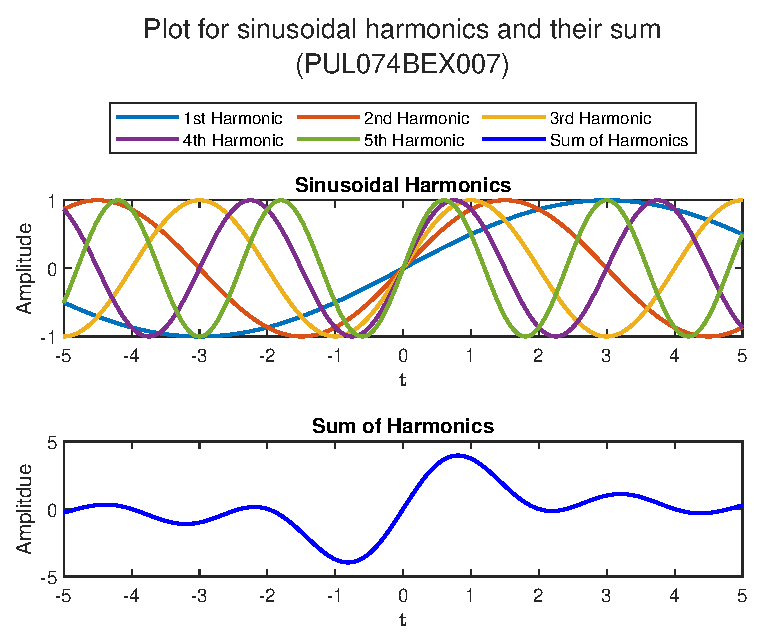
\includegraphics[width=0.85\linewidth]{../Figures/lab_2_5.eps}
    \caption{Plot for sinusoidal harmonics and their sum}
    \label{fig:2_5}
\end{figure}
\end{document}